
\chapter{Aufgabe D6}
Statt der aufgezeichneten Daten werden nun die Geschwindigkeiten aus dem Randomgenerator genutzt, um das Modell zu prüfen. \\
Eingestellt werden kann für den Randomgenerator zum einen die Basisgeschwindigkeit, um die durch den Randomgenerator Noise generiert werden kann. Sowie das Noiselevel/Amplitude, das das generierte Signal haben soll. Im Folgenden ist ein Ausschnitt zu sehen, wie der Randomgenerator  in das bestehende Modell integriert wird, sowie die erzeugten Daten des Randomgenerators und ob es Imbalancen im System mit dem Randomgenerator gibt.
\begin{figure}[H]
	\centering
	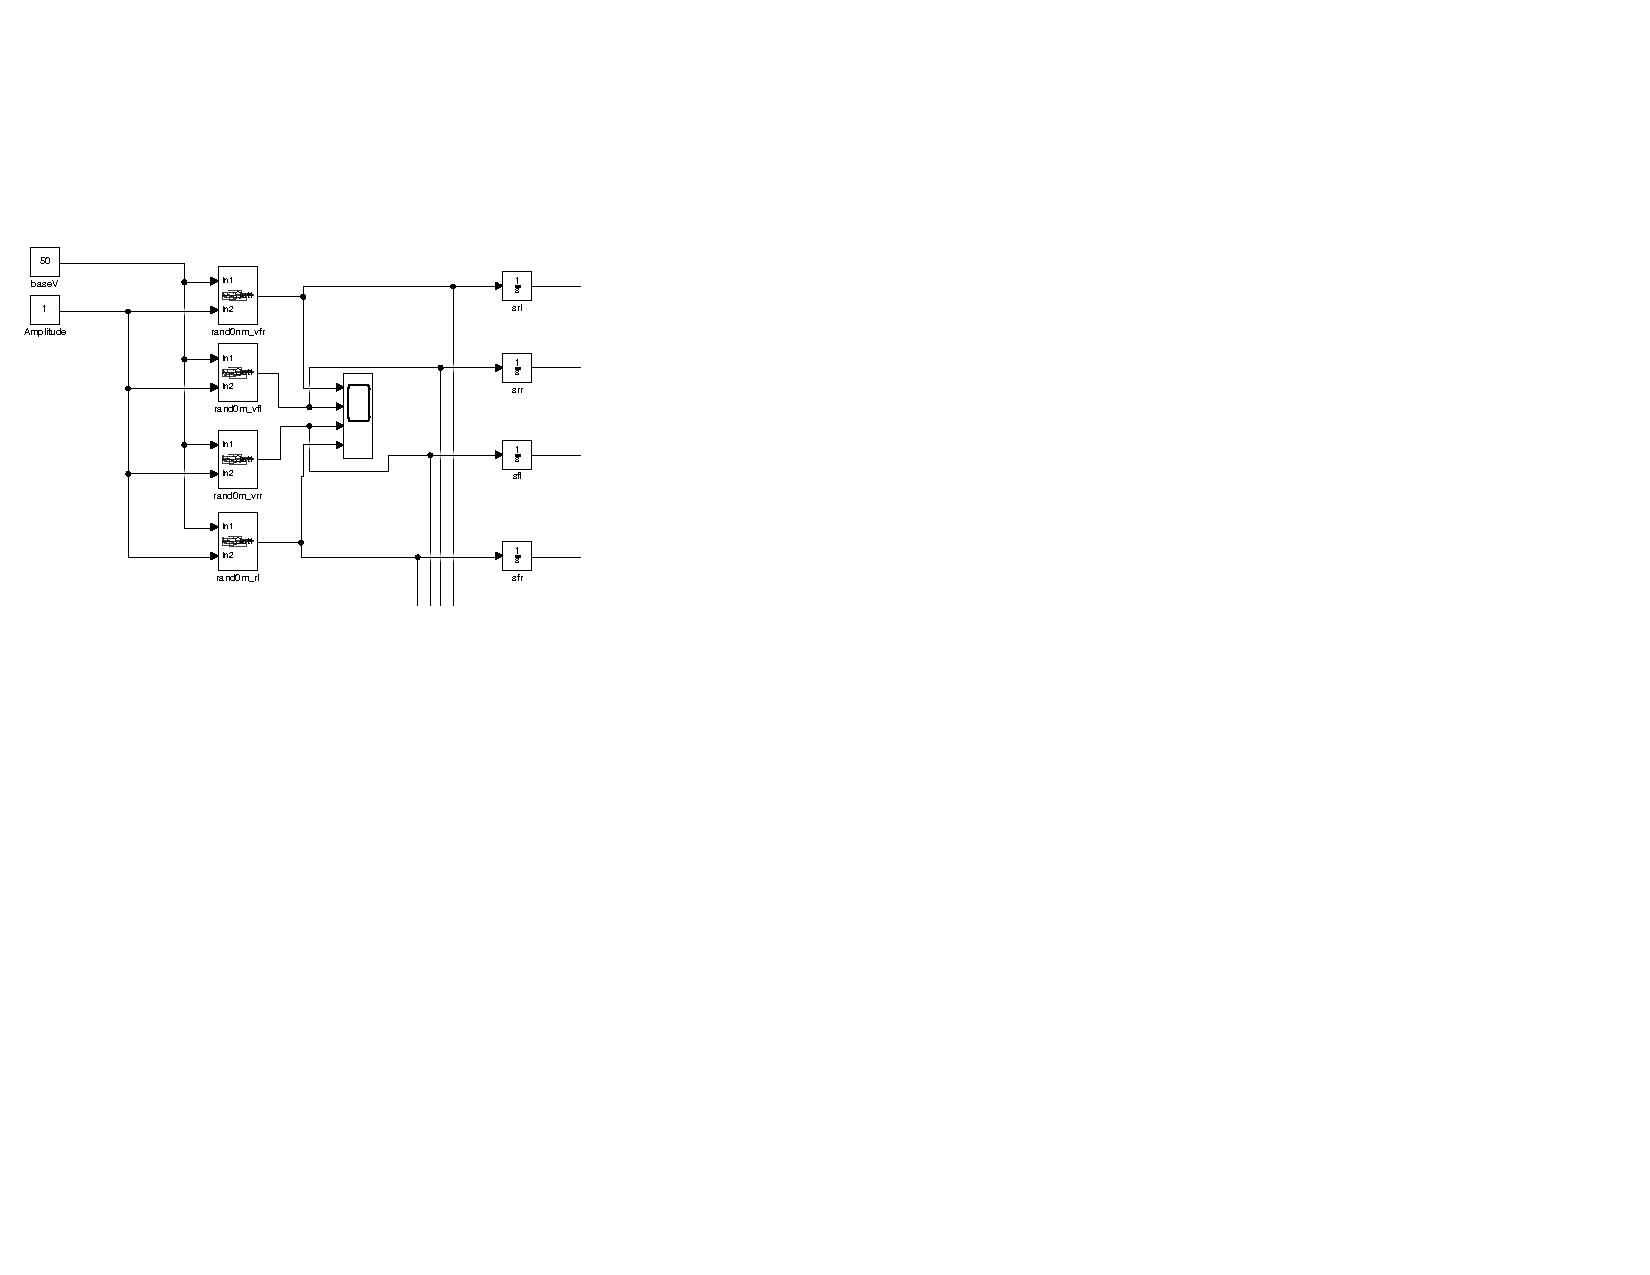
\includegraphics[width=0.95\linewidth]{../Graphiken/TireSimRandom}
	\caption{Include Random Generator}
	\label{fig:randomGeneratorAusschnitt}
\end{figure}
\begin{figure}[H]
	\centering
	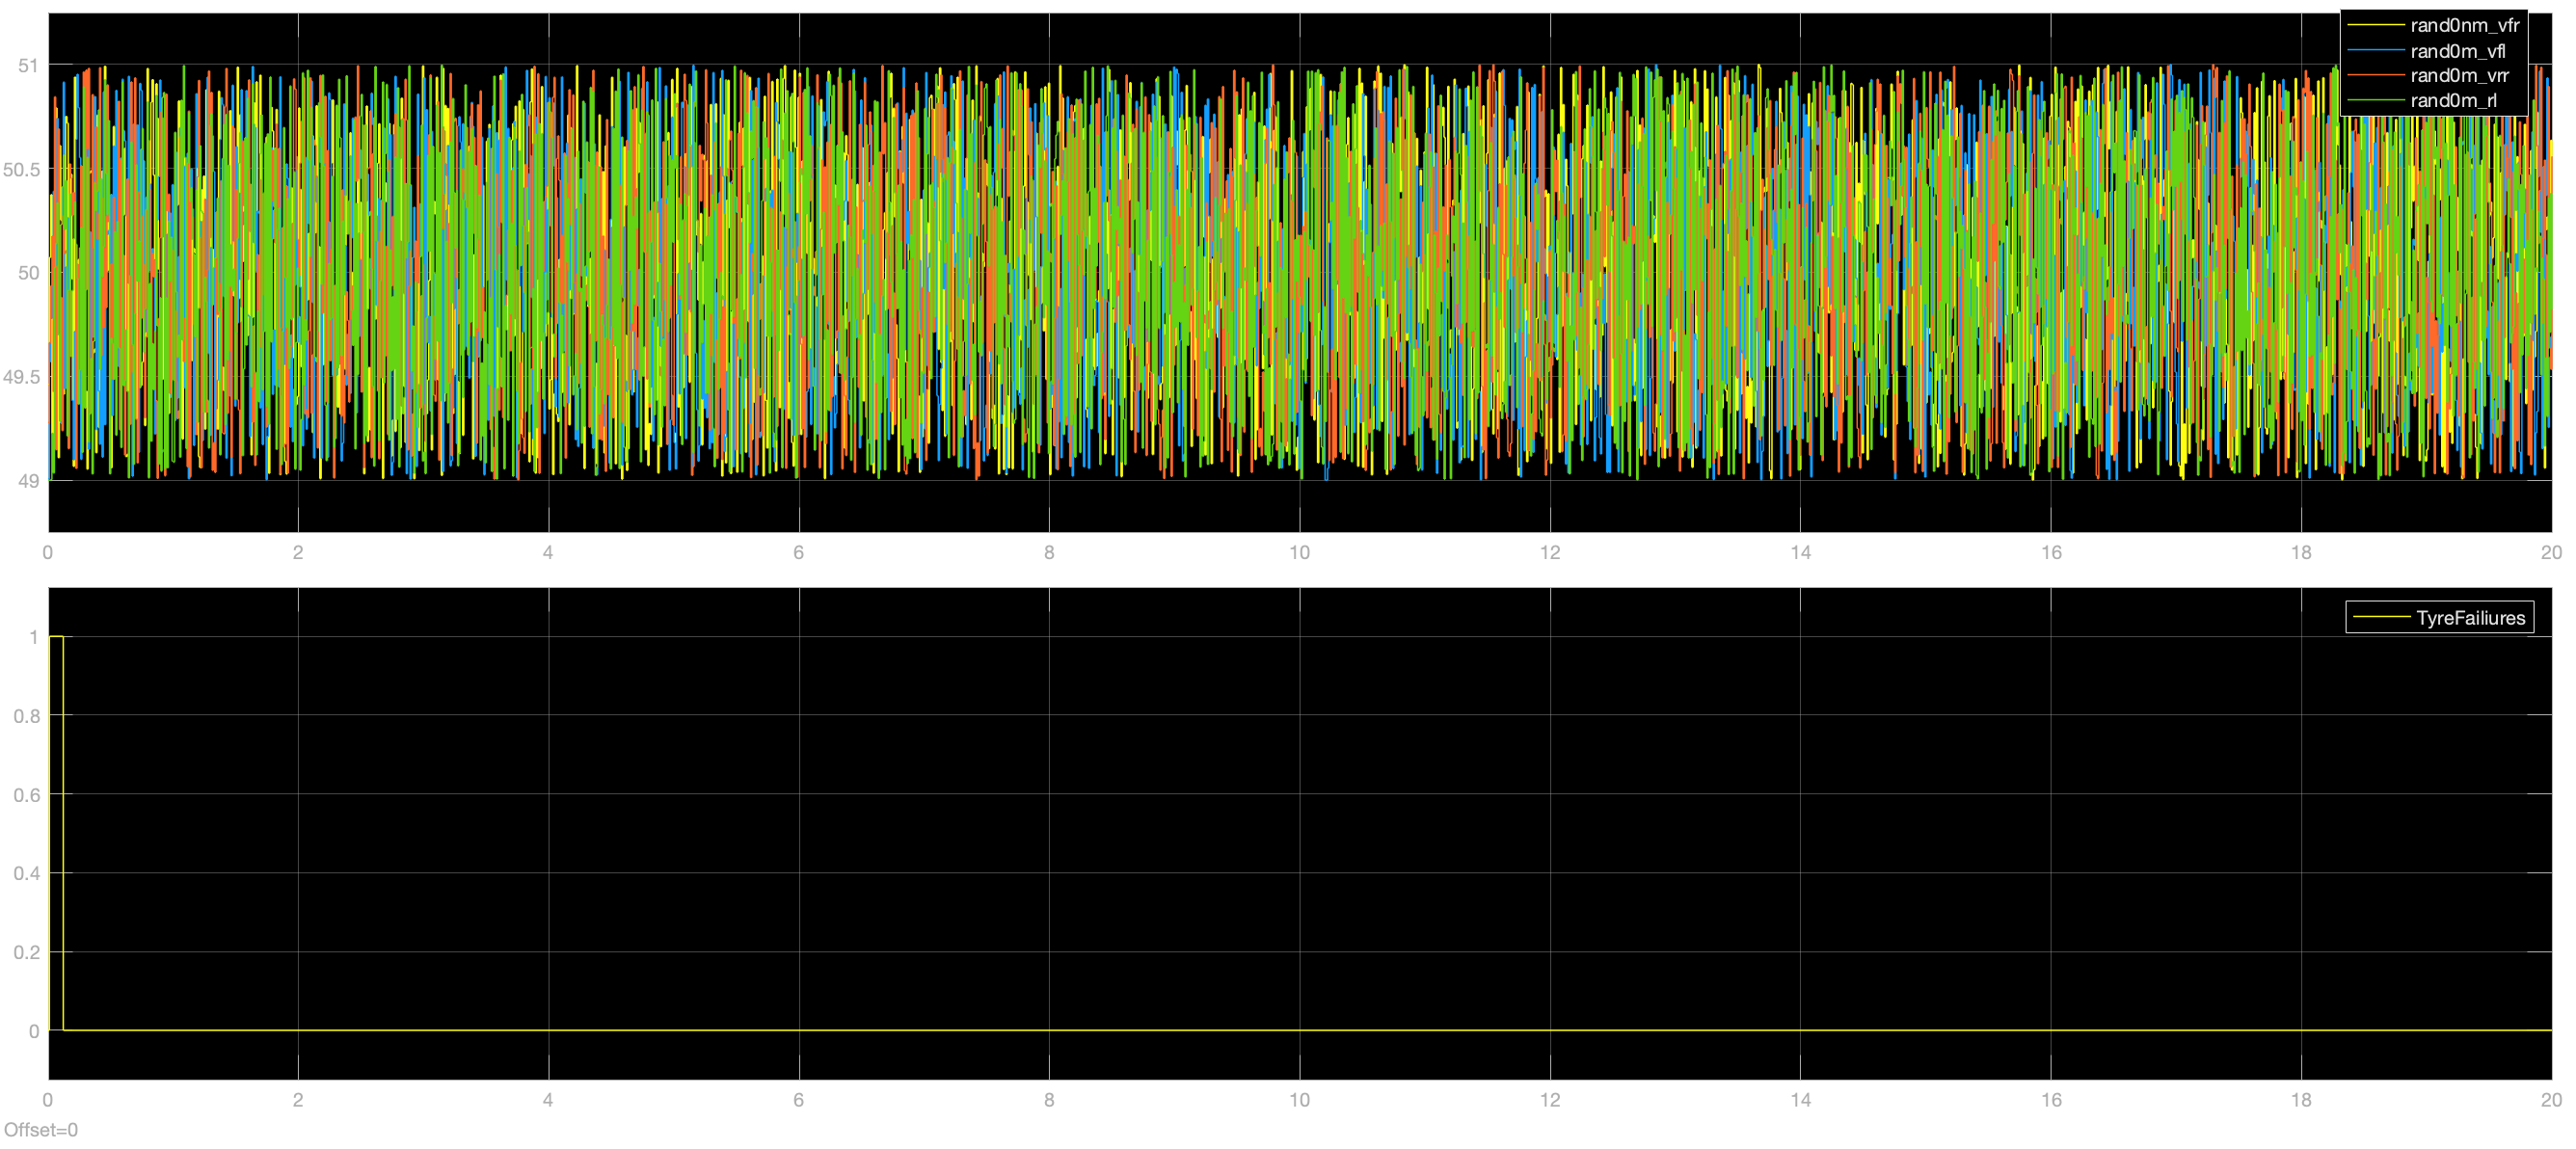
\includegraphics[width=0.95\linewidth]{../Graphiken/RandomGeneratorData}
	\caption{Generated Data}
	\label{fig:randomgeneratordata}
\end{figure}
Es wird deutlich, dass es keine Imbalancen bei diesem Beispiel gibt, auch bei anderen Basisgeschwindigkeiten und anderen Noiseleveln, die einer realistischen Geradeausfahrt entsprechen treten keine Imbalancen auf.\\
Damit ist der konstruierte Randomgenerator gut geeignet, um Geradeausfahrten zu simulieren.
